\documentclass[a4paper,11pt, twocolumn]{article}
\usepackage[margin=0.5in]{geometry}
\usepackage{graphicx}
\usepackage[font={small,it}]{caption}
\usepackage{wrapfig}
\usepackage{amsmath}
\usepackage{amssymb}
\usepackage{hyperref}

\begin{document}

\title{Linear Regression on Boston Housing Data}
\author{Alun Meredith}
\maketitle
\begin{abstract}

In this lab we explore the use of linear regression to predict housing prices on the Boston Housing data from the UCI Machine Learning repository *** REF. 

We describe linear regression and different techniques such as gradient descent and varying the cost function on it.  

Finally we discuss different errors in our model produced by bias and variance and methods to reduce these errors such as cross validation and regularisation. 
\end{abstract}

\section{Linear Regression}
Linear regression is the attempt to fit a linear model of the form of equation \ref{eq:1} to training data. This model is parametrised  by the intercept $x_0$ and the gradient vector $\mathbf{\theta}$. 
\begin{align}
	f = \mathbf{\theta}^t\mathbf{\theta} + x_0
	\label{eq:1}
\end{align}

Similarly to some of the linear classifier methods used previously we minimise a cost function based on the difference between our model and the data points (residuals) to produce the best linear fit. 

There are different choices for cost function based on how much weight you want to give different types of errors and the computational requirements. The earliest and most common estimation for error is the least square error where the we minimise the sum of the residuals squared. This error model is computationally convenient \ref{eq:3} and corresponds to a Gaussian model for the noise producing the errors. This means that data far away from the model is exponentially unlikely, to evaluate if this is a good model is a good fit we could look at the distribution of residuals and compare it to a normal distribution. 

Finally by normalising by the degrees of freedom we get the mean square error (MSE) and its square root (RMSE), an estimate for variance/standard deviation in the Gaussian population error. This is also useful as a single numerical value to evaluate the performance of our model.

\begin{align}
	J(\theta) = MSE = \frac{1}{n-2}  \sum^n_{i=1} (y_n^t\theta - f_n)^2
	\label{eq:2}
\end{align}

To find the value of $\theta$ which minimises $J(\theta)$ differentiate with respect to theta and set to zero $ (\frac{\partial J}{\partial \theta_i} = 0)$ and evaluate the value of theta which satisfies this equation. This produces a number of simultaneous equations based on the number of variables being minimised $(p+1)$ which must be solved. 

For this particular cost function (eq.\ref{eq:2}) we can solve these linear functions using the pseudo-inverse to evaluate the values of $\theta$ which minimise the cost function:

\begin{align}
	\theta = y^tX(X^tX)^{-1}
	\label{eq:3}
\end{align}

Before performing these techniques on the Boston Housing data, the data was first normalised. This involves artificially setting the mean of each variable to 0 and variance to 1. This prevents variables with large numbers dominating the cost equation and having unfair weight to the final optimisation. 

After performing the linear regression method described a model of normalised house value is plotted against the true value in figure \ref{fig:1}. The line $y=x$ describes accurate predictions. The figure shows the data generally groups around that line but high true house prices pull away from this model significantly. 

\begin{figure}[ht]
	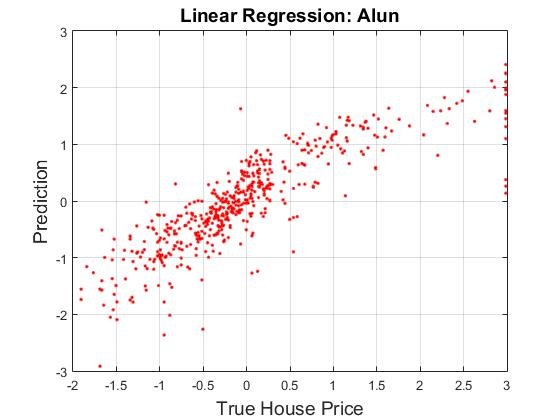
\includegraphics[width=0.8\linewidth]{figure1.jpg}
	\centering
	\caption{Prediction vs. true value of normalised house price}
		\label{fig:1}
\end{figure}

Looking at the distribution of the residuals (fig.\ref{fig:2}) in this prediction and  (fig.\ref{fig:1}) we can see non-negligible houses at the extreme value of price which breaks our expected Gaussian residuals using the MSE. To compensate for this it may be better to use a different cost function or we could just remove these data points as outliers. 

\begin{figure}[ht]
	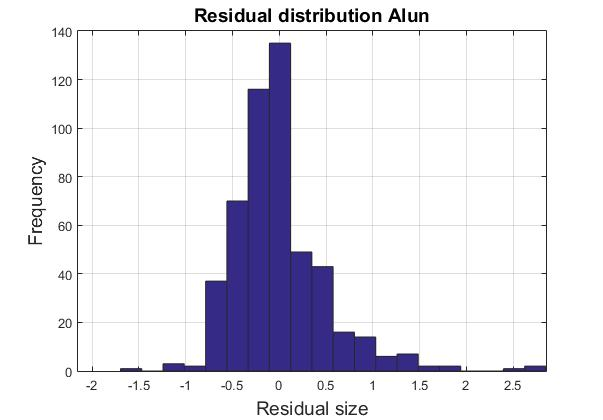
\includegraphics[width=0.8\linewidth]{figure2.jpg}
	\centering
	\caption{Distribution in residuals}
		\label{fig:2}
\end{figure}

By splitting the data into a training set and a testing set we can evaluate the performance of the linear regression. Evaluating the RMSE on both the training set and testing set over 10 runs we achieve an RMSE of only 0.117 this is a very low error value but doesn't tell us much about how well our model fits new data, for that a testing set was used and gave an error of 2.663/. \footnote{numbers extracted from average validation set error in cross validation so more directly comparable} The large difference between test set and training set error suggests that our model has overfit the training set producing an overly complex model which doesn't generalise well. 
\section{Variance}
By default our model produces complex linear solutions in order to best fit the training data. This produces the lowest possible training error but the solutions can vary a lot with small changes in the training data and therefore poor relative performance of the testing data. This effect is known as variance. To reduce the effect of variance on the data large datasets are often used. A useful to reduce the effect of variance is also k-fold validation.

K-fold validation is the concept of splitting the data into k different sets. Each set is used as a testing set once while the rest of the data is used for training data. This is repeated for each fold so we have k models of the data. These models are averaged to create a more generalised model.

It is important to set aside a testing set which isn't part of any validation or training set so that generalisation error of the final model can still be computed. Using 10 fold cross validation we achieve a generalisation (test set) error of 0.652 which is much better than before. 
\section{Regularisation}
\section{Gradient Descent}
Although the cost function that we have used can be solved through the pseudo-inverse method described by equation \ref{eq:3}, often the data set is either too large to calculate efficiently in this manner or another cost function without an easy computational trick like this is being used. If this is the case a method called gradient descent is used. Gradient descent calculates the gradient at a point and moves down the gradient by an amount (learning rate = $\alpha$). This can find a minima for the gradient very quickly, although it can sometimes find a local minima and not the global minimum so often the process randomly reinitialised several times when the gradient of the cost function can have local minima. 

Using a gradient descent algorithm a linear model was trained, producing figure \ref{fig:3}. 

** table training error 0.117, validation error 2.663, test error 0.652
\end{document}
